\pagebreak
\abstract{This manual provides user information for the AVNA1 Audio Test Instrument. Detailed information on using the capabilities are provided along with some background and technical details.  This manual  is in support of the main web page,\linebreak  \textbf{\texttt{http://www.janbob.com/electron/AVNA1/AVNA1.htm}}.  \linebreak The origins of this project go back to an QEX article, \linebreak \textbf{\texttt{\small{http://www.janbob.com/electron/AVNA1/Larkin-QEX-2018-May-Jun.pdf}}}.

\section{Features and Capabilities}
The capabilities of Version 0.82 and following versions are the following:
\begin{itemize}
\item Audio Impedance Measurement
\item Audio Vector Network Analyzer (Audio Transmission Measurements)
\item Audio Spectrum Analyzer covering up to 40 kHz with graphical display
\item Vector Voltmeter with frequency selectivity and adjustable phase offset
\item Four Signal Generators (added together)  with calibrated output.
\item Weighted and Unweighted Noise Measurement
\item Envelope and Group Delay Measurement
\item Screen Save to BMP file for all functions
\item Calibration of input and output levels and for the touch screen
\item AVNA Control via Serial Port
\end{itemize}

\subsection{Terminology in this Manual}This User's Manual covers the use of the AVNA1 to make the various measurements.  Before getting into the details, a couple of notes about terminology may be useful.  First, the term "AVNA1" refers to this specific hardware and software making up the project first published in QEX.  The AVNA part, of course, refers to Audio Vector Network Analyzer.  Since the project was published, several other instrument functions have been added, as listed with the bullets above.  This has suggested the need for a new name, and so in this manual we will refer to "Audio Test Instrument."  The project name remains "AVNA1."   The specific instruments have separate sections covering their operation.

\subsection{Terminal Terminology}There are two sets of physical terminals:
\begin{enumerate}
\item The impedance measuring pair of terminals are also used anytime there is an output signal.   Because of the original use of these terminals, we refer to the connector by \q{Z}, the commonly used impedance symbol.  The output resistance is software controlled at either 50 or 5000 Ohms, depending on the application.
\item The transmission input pair of terminals are always used when a signal is coming into the AVNA1.  Following the same logic, we refer to this pair of terminals by \q{T}.  The input impedance is either 1 Megohm in parallel with 25 pF or 50 Ohms, depending on the 50-Ohm switch.
\end{enumerate}
In addition to the \q{Z} and \q{T} terminals there is a signal output, usually on a BNC connector, that has an output impedance close to zero Ohms.  This is used for specialized purposes and always has the same signal applied to it as the\q{Z} terminals.

\section{Power Up}
\label{sect:PwrUp}
When the AVNA1 is turned on, it starts with an "Audio Test Instrument" screen that allows selection of the function.  This is, as usual, selected by the six touch screen buttons at the bottom of the screen.  In addition, if an $\mu$SD card is present in the Teensy 3.6 socket, a button with "\textsf{S}"  shows in the upper right corner for "Screen Save".

\begin{figure}[H]
\begin{center}
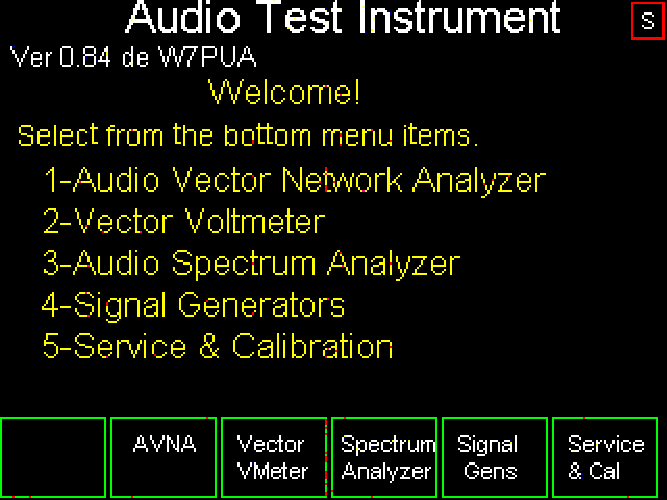
\includegraphics[scale=0.75]{./images/AVNA_000.pdf}
\caption{Power-up Screen}
\label{power-up-label}
\end{center}
\end{figure}

At startup, the Serial Monitor shows the status of the $\mu$SD card followed by a directory listing. For example:
\textsf{
\begin{itemize}
  \item Initializing SD card...and a card is present.
  \item Partition found: FAT32
  \item Volume size (Mbytes): 7378
  \item Files found on the card (name, date, time, and size in bytes):
  \begin{itemize}
   \item AVNA1\_00.BMP  2000-01-01 01:00:00 230454
   \item AVNA1\_01.BMP  2000-01-01 01:00:00 230454
   \end{itemize}
\end{itemize}}

\textbf{Note:} $\mu$SD cards have grown in GB capacity over the years.  There may be problems with large capacity cards greater than 8 GB.
